\documentclass[11pt, a4paper]{article}
\usepackage[utf8]{inputenc}
\usepackage{minted}
\usepackage{graphicx}
\usepackage{hyperref}
\graphicspath{{./images/}}

\begin{document}
\title{Transfer Learning}
\author{Samuel Navarro}
\date{\today}
\maketitle
\tableofcontents{}
	


\section{Transfer Learning}%
\label{sec:transfer_learning}

Depending on both:
\begin{itemize}
	\item The size of the new data set, and
	\item The similarity of the new data set to the original data set
\end{itemize}


The approach for using transfer learning will be different. There are four main cases:

\begin{enumerate}
	\item New data set is small, new data is similar to original training data.
	\item New data set is small, new data is different from original training data.
	\item New data set is large, new data is similar to original training data.
	\item New data set is large, new data is different from original training data.
\end{enumerate}



\begin{figure}[htpb!]
	\centering
	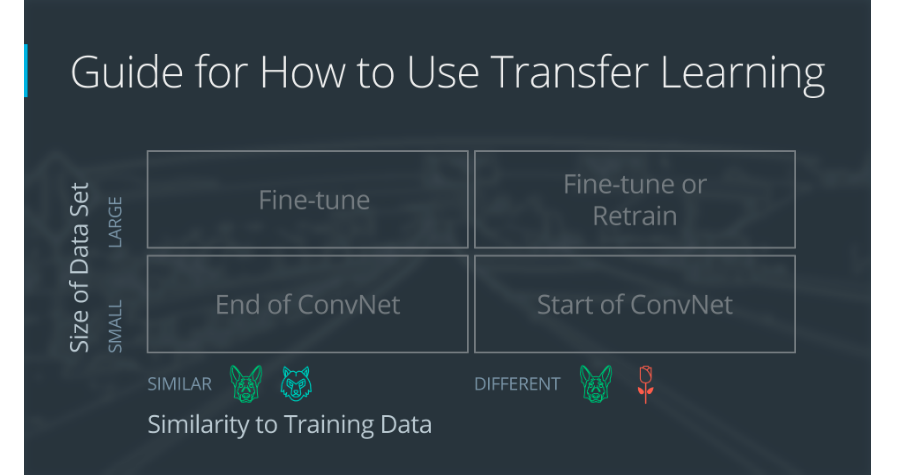
\includegraphics[width=0.8\linewidth]{transfer_learning_guide}
	\caption{Transfer Learning Guide}
	\label{fig:transfer_leraning_guide}
\end{figure}


\textbf{Overfitting} is a concern when using transfer learning with a small data set.



\subsection{Demonstration Network}%
\label{ssub:demonstration_network}

Our example network contains three convolutional layers and three fully connected layers:



\begin{figure}[htpb!]
	\centering
	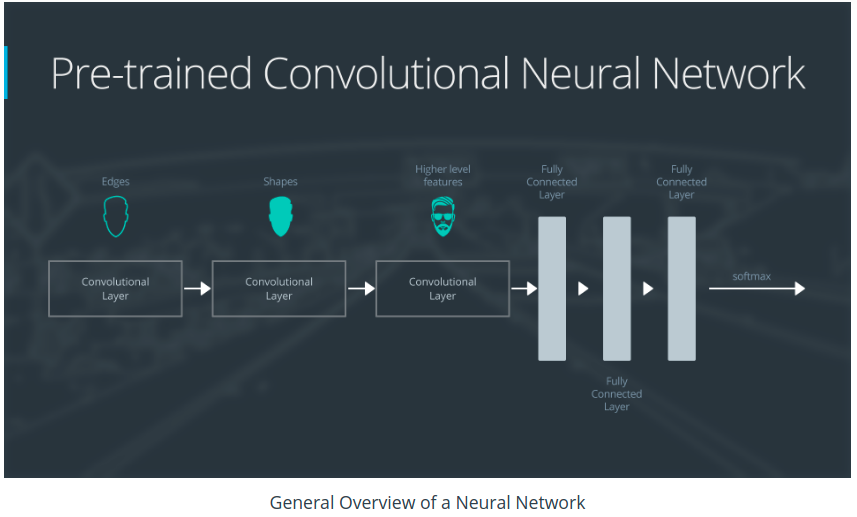
\includegraphics[width=0.8\linewidth]{pretrained_convnet}
	\caption{Pretrained ConvNet}
	\label{fig:pretrained_convnet}
\end{figure}





Each \textbf{transfer learning} case will use the pre-trained convolutional neural network in a different way.



\subsubsection{Case1: Small Data Set, Similar Data}%
\label{ssub:case1_small_data_set_similar_data}


If the data set is small and similar to the original training data:

\begin{itemize}
	\item Slice off the end of the neural network.
	\item Add a new fully connected layer that matches the number of classes in the new data set.
	\item Randomize the weights of the new fully connected layer; freeze all the weights from the pretrained network.
	\item Train the network to update the weights of the new fully connected layer.
\end{itemize}


To avoid overfitting on the small data set, the weights of the original network will be held constant rather than re-training the weights.

Since the data sets are similar, images form each data set will have similar higher level features. Therefore most or all of the pre-trained neural network layers already contain relevant information about the new data set and should be kept.


\begin{figure}[htpb!]
	\centering
	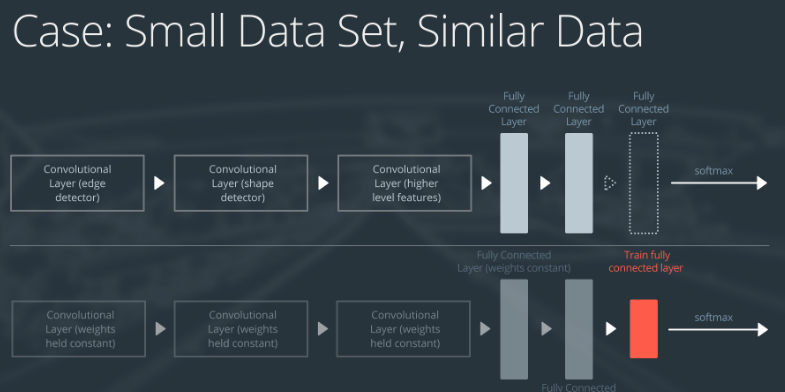
\includegraphics[width=0.8\linewidth]{small_dataset_similar_data}
	\caption{Small Dataset Similar Data}
	\label{fig:small_dataset_similar_data}
\end{figure}



\subsubsection{Case 2: Small Data Set, Different Data}%
\label{ssub:case_2_small_data_set_different_data}



If the new data set is small and different from the original training data:


\begin{itemize}
	\item Slice off most of the pre-trained layers near the beginning of the network.
	\item Add to the remaining pre-trained layers a new fully connected layer that matches the number of classes in the new data set.
	\item Randomize the weights of the new fully connected layer; freeze all the weights from the pre-trained network
	\item Train the network to update the weights of the new fully connected layer
\end{itemize}


Because the data set is small, \textbf{overfitting} is still a concern. To combat overfitting, the weights of the original neural network will be held constant, like in the first case. 

But the original training set and the new data set do not share higher level features. In this case, the new network will only use the layers containing lower level features.


\begin{figure}[htpb!]
	\centering
	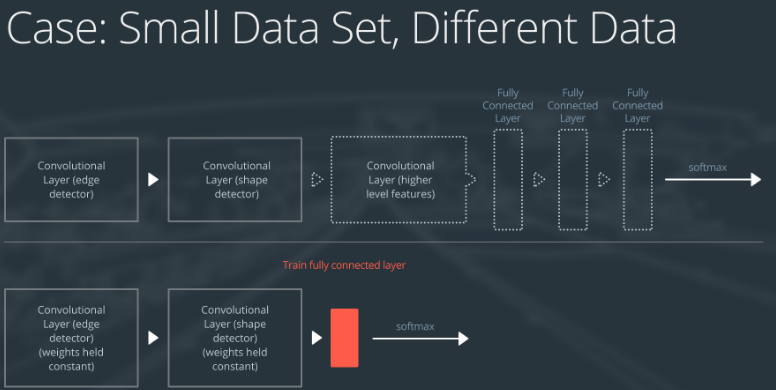
\includegraphics[width=0.8\linewidth]{small_dataset_different_data}
	\caption{Small Dataset, Different Data}
	\label{fig:small_dataset_different_data}
\end{figure}



\subsubsection{Case 3: Large Data Set, Similar Data}%
\label{ssub:large_data_set_similar_data}

If the new data set is large and similar to the original training data:

\begin{itemize}
	\item remove the last fully connected layer and replace with a layer matching the number of classes in the new data set.
	\item Randomly initialize the weights in the new fully connected layer
	\item Initialize the rest of the weights using the pre-trained weights
	\item re-train the entire neural network
\end{itemize}

Overfitting is not as much of a concern when training on a large data set; therefore, you can re-train all of the weights. Because the original training set and the new dta set share higher level features, the entire neural network is used. 



\begin{figure}[htpb!]
	\centering
	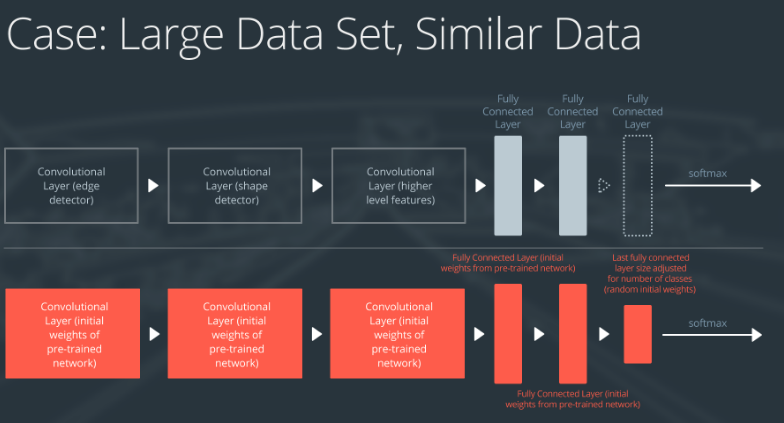
\includegraphics[width=0.8\linewidth]{large_dataset_similar_data}
	\caption{Large Dataset Similar Data}
	\label{fig:large_dataset_similar_data}
\end{figure}


\subsubsection{Case 4: Large Data Set, Different Data}%
\label{ssub:large_data_set_different_data}

If the new data set is large and different from the original data:

\begin{itemize}
	\item Remove the last fully connected layer and replace with a layer matching the number of classes in the new data set
	\item Retrain the network from scratch with randomly initialized weights.
	\item Alternatively, you could just use the same strategy as the \textit{large and similar} data case. 
\end{itemize}




\begin{figure}[htpb!]
	\centering
	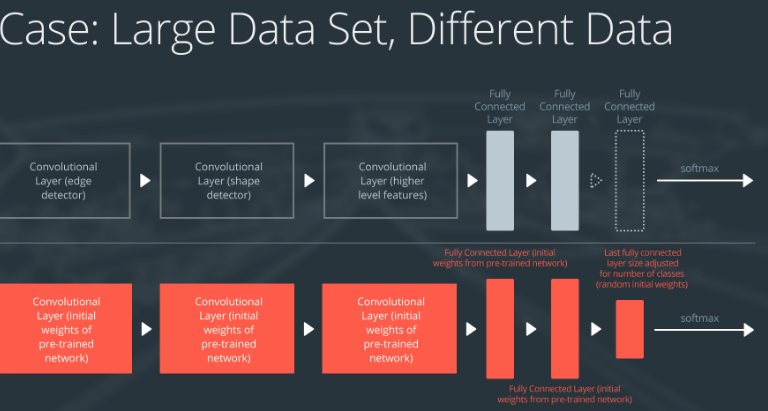
\includegraphics[width=0.8\linewidth]{large_dataset_different_data}
	\caption{Large Dataset, Different Data}
	\label{fig:large_dataset_different_data}
\end{figure}





\subsection{Popular Architectures}%
\label{sub:popular_architectures}


\subsubsection{AlexNet}%
\label{ssub:alexnet}

\textbf{AlexNet} puts the network on two GPUs. Although most of the calculations are done in parallel, the GPUs communicate with each other in certain layers. The original paper on AlexNet said that parallelizing the network decreased the classification error rate by 1.7\% when compared to a neural network that used half as may neurons on one GPU.





\begin{figure}[htpb!]
	\centering
	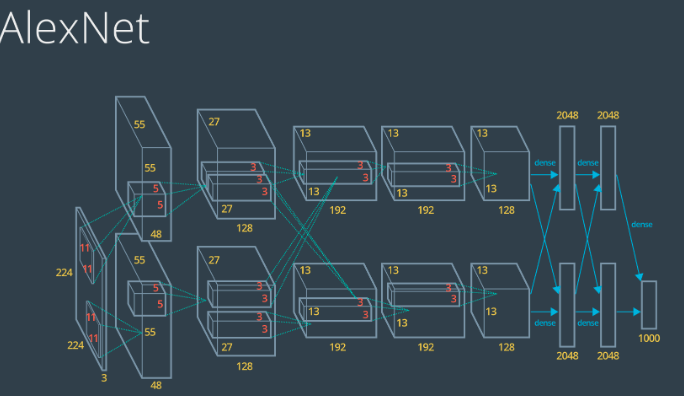
\includegraphics[width=0.8\linewidth]{alexnet}
	\caption{AlexNet Architecture}
	\label{fig:alexnet}
\end{figure}



\textbf{AlexNet} is still used today as a starting point for building and training neural networks. Actually, sometimes the researchers uses a small version of AlexNet because they discovered they some features of the AlexNet wasn't necessary. 





\subsubsection{VGG}%
\label{ssub:vgg}



\href{https://arxiv.org/pdf/1409.1556.pdf}{Here is the VGG Paper}


Is a large and elegant Architecture which makes it great for transfer learning. It is just a long sequence of three-by-three convolutions, broken up by two-by-two pooling layers and finished by a trio of fully connected layers at the end. 


\begin{figure}[htpb!]
	\centering
	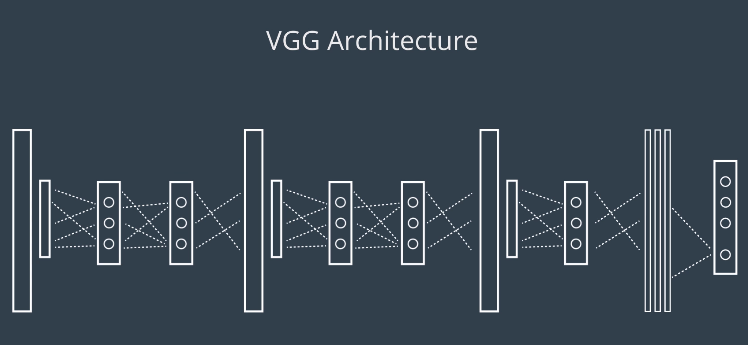
\includegraphics[width=0.8\linewidth]{vgg}
	\caption{VGG}
	\label{fig:vgg}
\end{figure}


Lot's of engineers uses VGG as a starting point for other image classification tasks. 


There are actually two versions of VGG, VGG16 and VGG19 (where the numbers denote the number of layers included in each respective model).


\begin{listing}
\begin{minted}[linenos,numbersep=5pt,frame=lines,framesep=2mm]{python}
from keras.applications.vgg16 import VGG16

model = VGG16(weights='imagenet', include_top=False)
\end{minted}
\caption{caption name}
\label{lst:caption_name}
\end{listing}


The argument \texttt{weights='imagenet'} loads the pre-trained ImageNet weights. You can also specify \texttt{None} to get random weights if you just want the architecture of \textbf{VGG16}. The argument \texttt{include\_top} is for whether you want to include the fully-connected layer at the top of the network; you likely want to set this to \texttt{False} unless you are actually trying to classify ImageNet's 1,000 classes.

VGG uses 224x224 images as input, so that's another thing to consider.






\begin{listing}
\begin{minted}[linenos,numbersep=5pt,frame=lines,framesep=2mm]{python}
from keras.preprocessing import image
from keras.applications.vgg16 import preprocess_input, VGG16, decode_predictions
import numpy as np

img_path = 'your_image.jpg'
img = image.load_img(img_path, target_size=(224, 224))
x = image.img_to_array(img)
x = np.expand_dims(x, axis=0)
x = preprocess_input(x)

model = VGG16(weights='imagenet')
predictions = model.predict(x)

print("Predicted:', decode_predictions(predictions, top=3)[0])

\end{minted}
\caption{caption name}
\label{lst:caption_name}
\end{listing}






\subsubsection{GoogLeNet}%
\label{ssub:googlenet}


\href{https://arxiv.org/pdf/1409.4842.pdf}{The paper of GoogleNet/Inception}


\textbf{GoogLeNet} great advantage is that it runs really fast. The team at google develop a concept called the Inception module, which trains really well and is efficiently deployable. 

The inception module creates a situation which the total number of parameters is very small and this is why \textbf{GoogLeNet} runs almost as fast as \textbf{AlexNet}. 
\textbf{GoogLeNet} is a great choice if you want to run your network in real time, like in a SelfDriving car.

In a normal \textbf{Inception Network}, you would see form the model summary that the last two layers were a global average pooling layers, and a fully-connected "Dense" layer. 

\textbf{Notes on Keras v.2.0.9:} 

\begin{enumerate}
	\item How many layers you drop is up to yo. We fropped the final two already by setting \texttt{include\_top} to False in the original loading of the model, but you could instead just run \texttt{pop()} twice to achieve similar results. \textit{Keras requires us to set include\_top to False in order to change the input\_shape}. Additional layers could be dropped by additional calls to \texttt{pop()}  
	\item If you make a mistake with \texttt{pop()} you'll want to reload the model. If you use it multiple times, the model will continue to drop more and more layers, so you may need to check \texttt{model.summary()} again. 
\end{enumerate}

The \href{https://keras.io/models/model/}{Model API} instead of using \texttt{model.add()} you explicitly tell the model which previous layer to attach to the current layer. This is useful is you want to use more advanced concepts like \href{https://en.wikipedia.org/wiki/Residual_neural_network}{skip layers} 


For example:

\texttt{x = Dropout(0.2)(inp)} is how you would attach a dropout with it's input coming from \texttt{inp}.


\textbf{Keras Callbacks}

Keras \href{https://keras.io/callbacks/}{callbacks}  allow you to gather and store additional information during training, such as the best model, or even stop training early if the validation accuracy has stopped improving. These methods can help to avoid overfitting, or avoid other issues.

There's two key callbacks to mention here, `ModelCheckpoint` and `EarlyStopping`. As the names may suggest, model checkpoint saves down the best model so far based on a given metric, while early stopping will end training before the specified number of epochs if the chosen metric no longer improves after a given amount of time.

To set these callbacks, you could do the following:

\texttt{checkpoint = ModelCheckpoint(filepath=save\_path, 
monitor='val\_loss', save\_best\_only=True)}



This would save a model to a specified \texttt{save\_path}, based on validation loss, and only save down the best models. If you set \texttt{save\_best\_only} to `False`, every single epoch will save down another version of the model.


\texttt{stopper = EarlyStopping(monitor='val\_acc', min\_delta=0.0003, patience=5)}


This will monitor validation accuracy, and if it has not decreased by more than 0.0003 from the previous best validation accuracy for 5 epochs, training will end early.


You still need to actually feed these callbacks into `fit()` when you train the model (along with all other relevant data to feed into `fit`):

\texttt{model.fit(callbacks=[checkpoint, stopper])}










\subsubsection{ResNet}%
\label{ssub:resnet}

The 2015 ImageNet winner was the \textbf{ResNet}. \href{https://arxiv.org/pdf/1512.03385.pdf}{Here's the paper}. It has 152 layers (for contrast, \textbf{AlexNet} has 8 layers. \textbf{VGG} has 19 layers and \textbf{GoogLeNet} has 22 layers. 


\begin{listing}
\begin{minted}[linenos,numbersep=5pt,frame=lines,framesep=2mm]{python}
from keras.applications.resnet50 import ResNet50
model = ResNet50(weights='imagenet', include\_top=False)
\end{minted}
\caption{caption name}
\label{lst:caption_name}
\end{listing}


\section{Further}%
\label{sec:further}


\subsection{Behavioral Cloning}%
\label{sub:behavioral_cloning}


The below paper shows one of the techniques Waymo has researched using imitation learning (aka behavioral cloning) to drive a car.

\href{https://arxiv.org/abs/1812.03079}{ChauffeurNet: Learning to Drive by Imitating the Best and Synthesizing the Worst} by M. Bansal, A. Krizhevsky and A. Ogale


Abstract: Our goal is to train a policy for autonomous driving via imitation learning that is robust enough to drive a real vehicle. We find that standard behavior cloning is insufficient for handling complex driving scenarios, even when we leverage a perception system for preprocessing the input and a controller for executing the output on the car: 30 million examples are still not enough. We propose exposing the learner to synthesized data in the form of perturbations to the expert's driving, which creates interesting situations such as collisions and/or going off the road. Rather than purely imitating all data, we augment the imitation loss with additional losses that penalize undesirable events and encourage progress -- the perturbations then provide an important signal for these losses and lead to robustness of the learned model. We show that the ChauffeurNet model can handle complex situations in simulation, and present ablation experiments that emphasize the importance of each of our proposed changes and show that the model is responding to the appropriate causal factors. Finally, we demonstrate the model driving a car in the real world.


\subsection{Object Detection and Tracking}%
\label{sub:object_detection_and_tracking}



The below papers include various deep learning-based approaches to 2D and 3D object detection and tracking.

\href{https://arxiv.org/abs/1512.02325}{SSD: Single Shot MultiBox Detector by W. Liu, et. al.}

Abstract: We present a method for detecting objects in images using a single deep neural network. Our approach, named SSD, discretizes the output space of bounding boxes into a set of default boxes over different aspect ratios and scales per feature map location. At prediction time, the network generates scores for the presence of each object category in each default box and produces adjustments to the box to better match the object shape. Additionally, the network combines predictions from multiple feature maps with different resolutions to naturally handle objects of various sizes. Our SSD model is simple relative to methods that require object proposals because it completely eliminates proposal generation and subsequent pixel or feature resampling stage and encapsulates all computation in a single network. [...] Experimental results [...] confirm that SSD has comparable accuracy to methods that utilize an additional object proposal step and is much faster, while providing a unified framework for both training and inference. Compared to other single stage methods, SSD has much better accuracy, even with a smaller input image size. [...]

\href{https://arxiv.org/abs/1711.06396}{VoxelNet: End-to-End Learning for Point Cloud Based 3D Object Detection by Y. Zhou and O. Tuzel}

Abstract: Accurate detection of objects in 3D point clouds is a central problem in many applications, such as autonomous navigation, housekeeping robots, and augmented/virtual reality. To interface a highly sparse LiDAR point cloud with a region proposal network (RPN), most existing efforts have focused on hand-crafted feature representations, for example, a bird's eye view projection. In this work, we remove the need of manual feature engineering for 3D point clouds and propose VoxelNet, a generic 3D detection network that unifies feature extraction and bounding box prediction into a single stage, end-to-end trainable deep network. [...] Experiments on the KITTI car detection benchmark show that VoxelNet outperforms the state-of-the-art LiDAR based 3D detection methods by a large margin. Furthermore, our network learns an effective discriminative representation of objects with various geometries, leading to encouraging results in 3D detection of pedestrians and cyclists, based on only LiDAR.

\href{http://openaccess.thecvf.com/content_cvpr_2018/papers/Luo_Fast_and_Furious_CVPR_2018_paper.pdf}{Fast and Furious: Real Time End-to-End 3D Detection, Tracking and Motion Forecasting with a Single Convolutional Net by W. Luo, et. al.}


Abstract: In this paper we propose a novel deep neural network that is able to jointly reason about 3D detection, tracking and motion forecasting given data captured by a 3D sensor. By jointly reasoning about these tasks, our holistic approach is more robust to occlusion as well as sparse data at range. Our approach performs 3D convolutions across space and time over a bird’s eye view representation of the 3D world, which is very efficient in terms of both memory and computation. Our experiments on a new very large scale dataset captured in several north american cities, show that we can outperform the state-of-the-art by a large margin. Importantly, by sharing computation we can perform all tasks in as little as 30 ms.


\subsection{Semantic Segmentation}%
\label{sub:semantic_segmentation}

\href{https://arxiv.org/abs/1511.00561}{SegNet: A Deep Convolutional Encoder-Decoder Architecture for Image Segmentation by V. Badrinarayanan, A. Kendall and R. Cipolla}


Abstract: We present a novel and practical deep fully convolutional neural network architecture for semantic pixel-wise segmentation termed SegNet. [...] The novelty of SegNet lies in the manner in which the decoder upsamples its lower resolution input feature map(s). Specifically, the decoder uses pooling indices computed in the max-pooling step of the corresponding encoder to perform non-linear upsampling. This eliminates the need for learning to upsample. The upsampled maps are sparse and are then convolved with trainable filters to produce dense feature maps. We compare our proposed architecture with the widely adopted FCN and also with the well known DeepLab-LargeFOV, DeconvNet architectures. This comparison reveals the memory versus accuracy trade-off involved in achieving good segmentation performance. [...] We show that SegNet provides good performance with competitive inference time and more efficient inference memory-wise as compared to other architectures. [...]















\end{document}
